\sectionthree{Deterministic Finite State Machines}
\begin{python0}
from solutions import *; clear()
\end{python0}

We need to formalize DFAs.

\begin{defn}
  A \defone{deterministic finite automata}
  (\sidebarskip{16pt}\defone{DFA})
  or a
  \sidebarskip{8pt}\defone{deterministic finite state machine}\sidebarskip{4pt}
  is defined by
  \[
  (\Sigma,Q,q_0,F,\delta)
  \]
  where
  \begin{tightlist}
  \item $\Sigma$ is a finite set called the
    \defone{alphabet}
  \item $Q$ is a set of \defone{states}
  \item $q_0 \in Q$ is the
    \defone{start state}
    or
    \sidebarskip{12pt}\defone{initial state}
  \item $F \subseteq Q$ is the set of 
    \defone{accept states}
    or
    \sidebarskip{18pt}\defone{final states}
  \item $\delta : Q \times \Sigma \rightarrow Q$ is the
    \defone{transition function}.
  \end{tightlist}
  In this case we will say that $M$ is defined over $\Sigma$.
\end{defn}

Note: In some books the ingredients
for a DFA is listed in this order $(Q, \Sigma, \delta, q_0, F)$
instead where the set of states come first.

\begin{center}
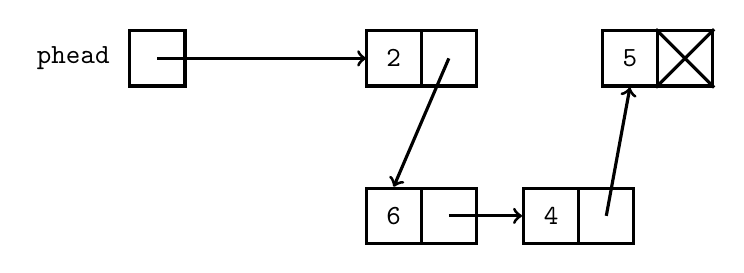
\begin{tikzpicture}

\draw (0.35, 0.35)
  node[draw, line width=0.04cm, , color=black,
       rounded corners=0cm, inner sep=0cm] {

\begin{minipage}[t][0.7cm]{0.7cm}
\mbox{}

\end{minipage}

};\draw (0.35, 0.35) node[color=black] {{\texttt{2}}};
\draw (1.0499999999999998, 0.35)
  node[draw, line width=0.04cm, , color=black,
       rounded corners=0cm, inner sep=0cm] {

\begin{minipage}[t][0.7cm]{0.7cm}
\mbox{}

\end{minipage}

};\draw (1.0499999999999998, 0.35) node[color=black] {{\texttt{}}};
\draw (0.35, -1.65)
  node[draw, line width=0.04cm, , color=black,
       rounded corners=0cm, inner sep=0cm] {

\begin{minipage}[t][0.7cm]{0.7cm}
\mbox{}

\end{minipage}

};\draw (0.35, -1.65) node[color=black] {{\texttt{6}}};
\draw (1.0499999999999998, -1.65)
  node[draw, line width=0.04cm, , color=black,
       rounded corners=0cm, inner sep=0cm] {

\begin{minipage}[t][0.7cm]{0.7cm}
\mbox{}

\end{minipage}

};\draw (1.0499999999999998, -1.65) node[color=black] {{\texttt{}}};
\draw (2.35, -1.65)
  node[draw, line width=0.04cm, , color=black,
       rounded corners=0cm, inner sep=0cm] {

\begin{minipage}[t][0.7cm]{0.7cm}
\mbox{}

\end{minipage}

};\draw (2.35, -1.65) node[color=black] {{\texttt{4}}};
\draw (3.0500000000000003, -1.65)
  node[draw, line width=0.04cm, , color=black,
       rounded corners=0cm, inner sep=0cm] {

\begin{minipage}[t][0.7cm]{0.7cm}
\mbox{}

\end{minipage}

};\draw (3.0500000000000003, -1.65) node[color=black] {{\texttt{}}};
\draw (3.35, 0.35)
  node[draw, line width=0.04cm, , color=black,
       rounded corners=0cm, inner sep=0cm] {

\begin{minipage}[t][0.7cm]{0.7cm}
\mbox{}

\end{minipage}

};\draw (3.35, 0.35) node[color=black] {{\texttt{5}}};
\draw (4.05, 0.35)
  node[draw, line width=0.04cm, , color=black,
       rounded corners=0cm, inner sep=0cm] {

\begin{minipage}[t][0.7cm]{0.7cm}
\mbox{}

\end{minipage}

};\draw (4.05, 0.35) node[color=black] {{\texttt{}}};\draw[line width=0.04cm,black,->] (1.05,0.35) to  (0.35,-1.28);
\draw[line width=0.04cm,black,->] (1.05,-1.65) to  (1.98,-1.65);
\draw[line width=0.04cm,black,->] (3.05,-1.65) to  (3.35,-0.02);
\draw[line width=0.04cm,black] (3.68,0.72) to  (4.42,-0.02);
\draw[line width=0.04cm,black] (4.42,0.72) to  (3.68,-0.02);

\draw (-2.65, 0.35)
  node[draw, line width=0.04cm, , color=black,
       rounded corners=0cm, inner sep=0cm] {

\begin{minipage}[t][0.7cm]{0.7cm}
\mbox{}

\end{minipage}

};\draw (-2.65, 0.35) node[color=black] {{\texttt{}}};\draw[line width=0.04cm,black,->] (-2.65,0.35) to  (0,0.35);

\draw (-3.7199999999999998, 0.35)
  node[draw, line width=0.04cm, , color=white,
       rounded corners=0cm, inner sep=0cm] {

\begin{minipage}[t][0.1cm]{0.1cm}
\mbox{}

\end{minipage}

};\draw (-3.7199999999999998, 0.35) node[color=black] {{\texttt{phead}}};
\end{tikzpicture}

\end{center}


%-*-latex-*-

\begin{ex} 
  \label{ex:prob-00}
  \tinysidebar{\debug{exercises/{disc-prob-28/question.tex}}}

  \solutionlink{sol:prob-00}
  \qed
\end{ex} 
\begin{python0}
from solutions import *
add(label="ex:prob-00",
    srcfilename='exercises/discrete-probability/prob-00/answer.tex') 
\end{python0}


\newpage
With the above formal definition of a DFA, we can now formally
define what we mean when we say that a string is accepted by a
DFA.

\begin{defn}
Let $M=(\Sigma,Q,q_0,F,\delta)$ be a DFA, $a\in\Sigma$ and $x \in
\Sigma^*$.
\begin{itemize}
  \item We write
   \[ (q,ax) \vdash (q',x) \]
   if
   \[ \delta(q,a) = q' \]
   i.e.,
   \[
   (q,ax) \vdash (\delta(q,a),x)
   \]
   This is a \textbf{computation} for string $ax$.
   The $(q, ax)$ and $(q', x)$ and in general
   the elements of $Q \times \Sigma^*$ are called
   \defone{instantaneous descriptions} (ID).
   Therefore $\vdash$ is a relation on $Q \times \Sigma^*$.
   You can think of $Q \times \Sigma^*$ as an infinite
   directed graph where the edges are determined by $\vdash$.

  \item We write
  \[ (q,x) \vdash^* (q',x') \]
  if either $(q,x) = (q',x')$ or there is a sequence of
  computations from $(q,x)$ to $(q',x')$:
  \[ (q,x) \vdash \cdots \vdash (q',x') \]
  In other words $\vdash^*$ is the \defterm{reflexive transitive
  closure} of $\vdash$.
\end{itemize}
\end{defn}


\begin{defn}
Given $x \in \Sigma^*$, we say that $x$ is
\defone{accepted} by $M$ iff
\[(q_0,x) \vdash^* (q',\ep) \quad \text{where \,} q' \in F \]
\end{defn}

\begin{center}
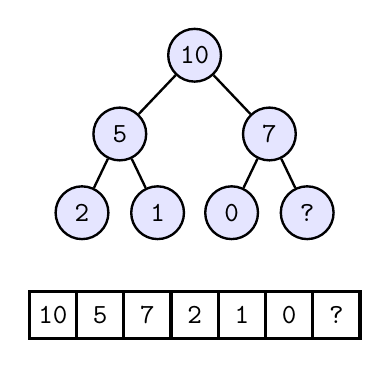
\begin{tikzpicture}

\fill[blue!10] (0.0, 0.0) circle (0.35);
\node [line width=0.03cm,black,minimum size=0.6699999999999999cm,draw,circle] at (0.0,0.0)(10){};\draw (0.0, 0.0) node[color=black] {\texttt{10}};
\fill[blue!10] (-0.95, -1.0) circle (0.35);
\node [line width=0.03cm,black,minimum size=0.6699999999999999cm,draw,circle] at (-0.95,-1.0)(5){};\draw (-0.95, -1.0) node[color=black] {\texttt{5}};
\fill[blue!10] (0.95, -1.0) circle (0.35);
\node [line width=0.03cm,black,minimum size=0.6699999999999999cm,draw,circle] at (0.95,-1.0)(7){};\draw (0.95, -1.0) node[color=black] {\texttt{7}};
\fill[blue!10] (-1.43, -2.0) circle (0.35);
\node [line width=0.03cm,black,minimum size=0.6699999999999999cm,draw,circle] at (-1.43,-2.0)(2){};\draw (-1.43, -2.0) node[color=black] {\texttt{2}};
\fill[blue!10] (-0.47, -2.0) circle (0.35);
\node [line width=0.03cm,black,minimum size=0.6699999999999999cm,draw,circle] at (-0.47,-2.0)(1){};\draw (-0.47, -2.0) node[color=black] {\texttt{1}};
\fill[blue!10] (0.47, -2.0) circle (0.35);
\node [line width=0.03cm,black,minimum size=0.6699999999999999cm,draw,circle] at (0.47,-2.0)(0){};\draw (0.47, -2.0) node[color=black] {\texttt{0}};
\fill[blue!10] (1.43, -2.0) circle (0.35);
\node [line width=0.03cm,black,minimum size=0.6699999999999999cm,draw,circle] at (1.43,-2.0)(?){};\draw (1.43, -2.0) node[color=black] {\texttt{?}};\draw[line width=0.03cm,black] (10) to  (5);
\draw[line width=0.03cm,black] (10) to  (7);
\draw[line width=0.03cm,black] (5) to  (2);
\draw[line width=0.03cm,black] (5) to  (1);
\draw[line width=0.03cm,black] (7) to  (0);
\draw[line width=0.03cm,black] (7) to  (?);

\draw (-1.8, -3.3)
  node[draw, line width=0.04cm, , color=black,
       rounded corners=0cm, inner sep=0cm] {

\begin{minipage}[t][0.6cm]{0.6cm}
\mbox{}

\end{minipage}

};\draw (-1.8, -3.3) node[color=black] {{\texttt{10}}};
\draw (-1.2, -3.3)
  node[draw, line width=0.04cm, , color=black,
       rounded corners=0cm, inner sep=0cm] {

\begin{minipage}[t][0.6cm]{0.6cm}
\mbox{}

\end{minipage}

};\draw (-1.2, -3.3) node[color=black] {{\texttt{5}}};
\draw (-0.6000000000000001, -3.3)
  node[draw, line width=0.04cm, , color=black,
       rounded corners=0cm, inner sep=0cm] {

\begin{minipage}[t][0.6cm]{0.6cm}
\mbox{}

\end{minipage}

};\draw (-0.6000000000000001, -3.3) node[color=black] {{\texttt{7}}};
\draw (-1.1102230246251565e-16, -3.3)
  node[draw, line width=0.04cm, , color=black,
       rounded corners=0cm, inner sep=0cm] {

\begin{minipage}[t][0.6cm]{0.6cm}
\mbox{}

\end{minipage}

};\draw (-1.1102230246251565e-16, -3.3) node[color=black] {{\texttt{2}}};
\draw (0.6, -3.3)
  node[draw, line width=0.04cm, , color=black,
       rounded corners=0cm, inner sep=0cm] {

\begin{minipage}[t][0.6cm]{0.6cm}
\mbox{}

\end{minipage}

};\draw (0.6, -3.3) node[color=black] {{\texttt{1}}};
\draw (1.2, -3.3)
  node[draw, line width=0.04cm, , color=black,
       rounded corners=0cm, inner sep=0cm] {

\begin{minipage}[t][0.6cm]{0.6cm}
\mbox{}

\end{minipage}

};\draw (1.2, -3.3) node[color=black] {{\texttt{0}}};
\draw (1.8, -3.3)
  node[draw, line width=0.04cm, , color=black,
       rounded corners=0cm, inner sep=0cm] {

\begin{minipage}[t][0.6cm]{0.6cm}
\mbox{}

\end{minipage}

};\draw (1.8, -3.3) node[color=black] {{\texttt{?}}};
\end{tikzpicture}

\end{center}


%-*-latex-*-

\begin{ex} 
  \label{ex:prob-00}
  \tinysidebar{\debug{exercises/{disc-prob-28/question.tex}}}

  \solutionlink{sol:prob-00}
  \qed
\end{ex} 
\begin{python0}
from solutions import *
add(label="ex:prob-00",
    srcfilename='exercises/discrete-probability/prob-00/answer.tex') 
\end{python0}


%-*-latex-*-

\begin{center}
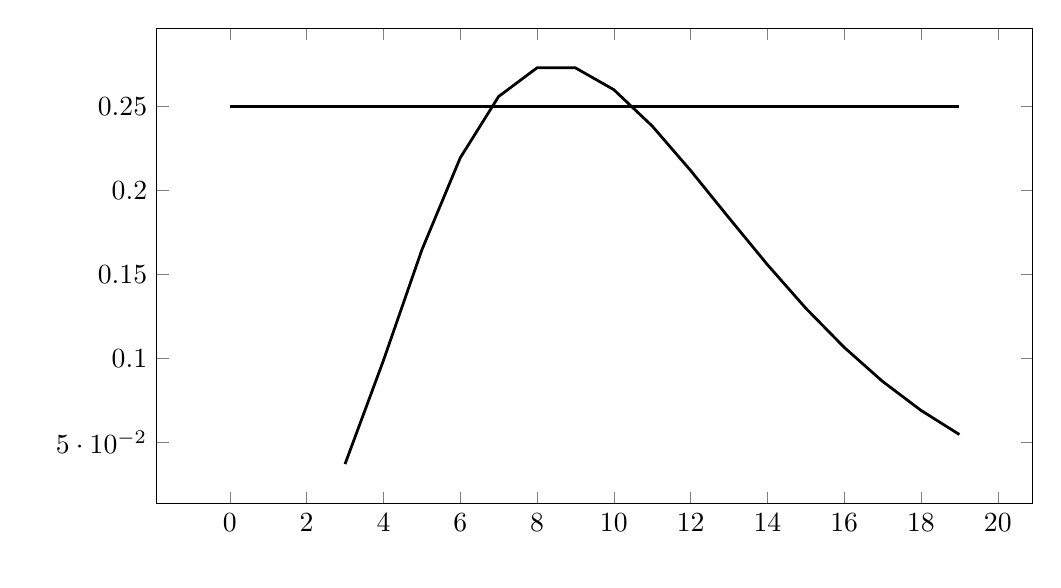
\begin{tikzpicture}[line width=1]
\begin{axis}[width=5in, height=3in,
             scatter/classes={a={mark=*,draw=black}},
             xlabel={\mbox{}},
             xlabel style={name=xlabel}, 
             ylabel={\mbox{}}, 
             legend style={
                at={(xlabel.south)},
                yshift=-1ex,
                anchor=north,
                legend cell align=left,
                },
        ]
]
\addplot[draw=black, line width=1] coordinates {(3, 0.03703703703703703)
(4, 0.0987654320987654)
(5, 0.16460905349794233)
(6, 0.21947873799725642)
(7, 0.2560585276634658)
(8, 0.2731290961743635)
(9, 0.2731290961743635)
(10, 0.26012294873748903)
(11, 0.23844603634269826)
(12, 0.2119520323046207)
(13, 0.18369176133067125)
(14, 0.15585967628056951)
(15, 0.12988306356714127)
(16, 0.10657071882432105)
(17, 0.08627153428635512)
(18, 0.06901722742908409)
(19, 0.05463863838135823)};\addplot[draw=black, line width=1] coordinates {(0, 0.25)
(1, 0.25)
(2, 0.25)
(3, 0.25)
(4, 0.25)
(5, 0.25)
(6, 0.25)
(7, 0.25)
(8, 0.25)
(9, 0.25)
(10, 0.25)
(11, 0.25)
(12, 0.25)
(13, 0.25)
(14, 0.25)
(15, 0.25)
(16, 0.25)
(17, 0.25)
(18, 0.25)
(19, 0.25)};
\end{axis}\end{tikzpicture}\end{center}

\begin{eg}
  using the $\vdash$ relation for the DFA
  Draw part of $Q \times \Sigma^*$ relation as a directed graph
Of course $Q \times \Sigma^*$ is infinite so you can't
draw the whole graph!
Just include $(q, x)$ for all $x$ with length $\leq 4$.
After that draw the relation for $\vdash^*$.
\end{eg}

\newpage
You can also define acceptance using an \lq\lq extension'' of $\delta$.
Note that the transition function basically defines one single
edge (transition) in the state diagram because the second input is a
character.
There is an obvious extension to $\delta$ so that the second
input is a string:

\begin{defn}
It is convenient to extend the transition function $\delta$ so that
we allow strings for the second argument instead of just character.
Define
\[
 \delta^* : Q \times \Sigma^* \rightarrow Q
\]
\begin{itemize}
 \item[(a)] $\delta^*(q, \ep) = q$ for all $q \in Q$
 \item[(b)] $\delta^*(q, ax) = \delta^*( \delta(a,q), x)$ for $a \in
 \Sigma$, $x \in \Sigma^*$, $q \in Q$.
\end{itemize}
\end{defn}


\begin{eg} Consider this DFA again:
\begin{center}
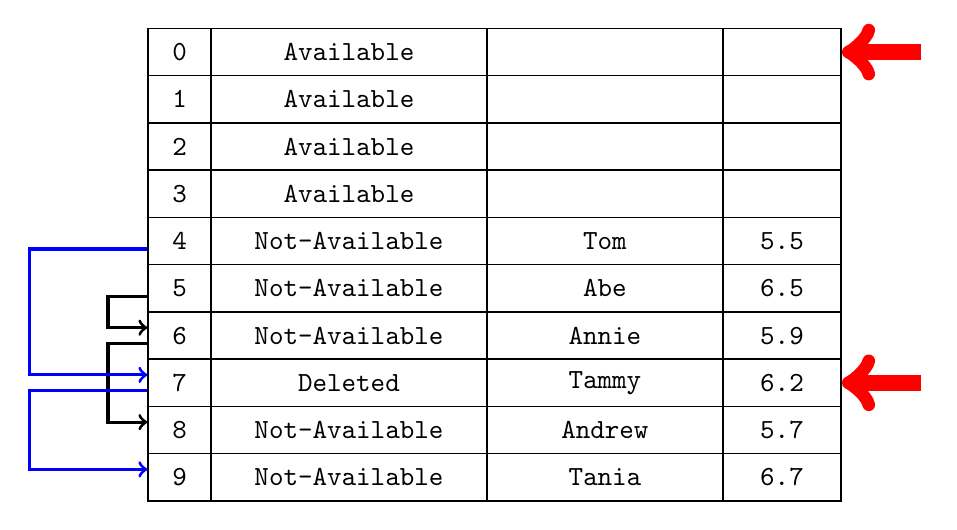
\begin{tikzpicture}

\draw (1.4, 0.7)
  node[draw, line width=0.02cm, , color=black,
       rounded corners=0cm, inner sep=0cm] {

\begin{minipage}[t][0.6cm]{0.8cm}
\mbox{}

\end{minipage}

};\draw (1.4, 0.7) node[color=black] {{\texttt{0}}};
\draw (3.55, 0.7)
  node[draw, line width=0.02cm, , color=black,
       rounded corners=0cm, inner sep=0cm] {

\begin{minipage}[t][0.6cm]{3.5cm}
\mbox{}

\end{minipage}

};\draw (3.55, 0.7) node[color=black] {{\texttt{Available}}};
\draw (6.800000000000001, 0.7)
  node[draw, line width=0.02cm, , color=black,
       rounded corners=0cm, inner sep=0cm] {

\begin{minipage}[t][0.6cm]{3.0cm}
\mbox{}

\end{minipage}

};\draw (6.800000000000001, 0.7) node[color=black] {{\texttt{}}};
\draw (9.05, 0.7)
  node[draw, line width=0.02cm, , color=black,
       rounded corners=0cm, inner sep=0cm] {

\begin{minipage}[t][0.6cm]{1.5cm}
\mbox{}

\end{minipage}

};\draw (9.05, 0.7) node[color=black] {{\texttt{}}};
\draw (1.4, 0.09999999999999987)
  node[draw, line width=0.02cm, , color=black,
       rounded corners=0cm, inner sep=0cm] {

\begin{minipage}[t][0.6cm]{0.8cm}
\mbox{}

\end{minipage}

};\draw (1.4, 0.09999999999999987) node[color=black] {{\texttt{1}}};
\draw (3.55, 0.09999999999999987)
  node[draw, line width=0.02cm, , color=black,
       rounded corners=0cm, inner sep=0cm] {

\begin{minipage}[t][0.6cm]{3.5cm}
\mbox{}

\end{minipage}

};\draw (3.55, 0.09999999999999987) node[color=black] {{\texttt{Available}}};
\draw (6.800000000000001, 0.09999999999999987)
  node[draw, line width=0.02cm, , color=black,
       rounded corners=0cm, inner sep=0cm] {

\begin{minipage}[t][0.6cm]{3.0cm}
\mbox{}

\end{minipage}

};\draw (6.800000000000001, 0.09999999999999987) node[color=black] {{\texttt{}}};
\draw (9.05, 0.09999999999999987)
  node[draw, line width=0.02cm, , color=black,
       rounded corners=0cm, inner sep=0cm] {

\begin{minipage}[t][0.6cm]{1.5cm}
\mbox{}

\end{minipage}

};\draw (9.05, 0.09999999999999987) node[color=black] {{\texttt{}}};
\draw (1.4, -0.5000000000000002)
  node[draw, line width=0.02cm, , color=black,
       rounded corners=0cm, inner sep=0cm] {

\begin{minipage}[t][0.6cm]{0.8cm}
\mbox{}

\end{minipage}

};\draw (1.4, -0.5000000000000002) node[color=black] {{\texttt{2}}};
\draw (3.55, -0.5000000000000002)
  node[draw, line width=0.02cm, , color=black,
       rounded corners=0cm, inner sep=0cm] {

\begin{minipage}[t][0.6cm]{3.5cm}
\mbox{}

\end{minipage}

};\draw (3.55, -0.5000000000000002) node[color=black] {{\texttt{Available}}};
\draw (6.800000000000001, -0.5000000000000002)
  node[draw, line width=0.02cm, , color=black,
       rounded corners=0cm, inner sep=0cm] {

\begin{minipage}[t][0.6cm]{3.0cm}
\mbox{}

\end{minipage}

};\draw (6.800000000000001, -0.5000000000000002) node[color=black] {{\texttt{}}};
\draw (9.05, -0.5000000000000002)
  node[draw, line width=0.02cm, , color=black,
       rounded corners=0cm, inner sep=0cm] {

\begin{minipage}[t][0.6cm]{1.5cm}
\mbox{}

\end{minipage}

};\draw (9.05, -0.5000000000000002) node[color=black] {{\texttt{}}};
\draw (1.4, -1.1000000000000003)
  node[draw, line width=0.02cm, , color=black,
       rounded corners=0cm, inner sep=0cm] {

\begin{minipage}[t][0.6cm]{0.8cm}
\mbox{}

\end{minipage}

};\draw (1.4, -1.1000000000000003) node[color=black] {{\texttt{3}}};
\draw (3.55, -1.1000000000000003)
  node[draw, line width=0.02cm, , color=black,
       rounded corners=0cm, inner sep=0cm] {

\begin{minipage}[t][0.6cm]{3.5cm}
\mbox{}

\end{minipage}

};\draw (3.55, -1.1000000000000003) node[color=black] {{\texttt{Available}}};
\draw (6.800000000000001, -1.1000000000000003)
  node[draw, line width=0.02cm, , color=black,
       rounded corners=0cm, inner sep=0cm] {

\begin{minipage}[t][0.6cm]{3.0cm}
\mbox{}

\end{minipage}

};\draw (6.800000000000001, -1.1000000000000003) node[color=black] {{\texttt{}}};
\draw (9.05, -1.1000000000000003)
  node[draw, line width=0.02cm, , color=black,
       rounded corners=0cm, inner sep=0cm] {

\begin{minipage}[t][0.6cm]{1.5cm}
\mbox{}

\end{minipage}

};\draw (9.05, -1.1000000000000003) node[color=black] {{\texttt{}}};
\draw (1.4, -1.7000000000000002)
  node[draw, line width=0.02cm, , color=black,
       rounded corners=0cm, inner sep=0cm] {

\begin{minipage}[t][0.6cm]{0.8cm}
\mbox{}

\end{minipage}

};\draw (1.4, -1.7000000000000002) node[color=black] {{\texttt{4}}};
\draw (3.55, -1.7000000000000002)
  node[draw, line width=0.02cm, , color=black,
       rounded corners=0cm, inner sep=0cm] {

\begin{minipage}[t][0.6cm]{3.5cm}
\mbox{}

\end{minipage}

};\draw (3.55, -1.7000000000000002) node[color=black] {{\texttt{Not-Available}}};
\draw (6.800000000000001, -1.7000000000000002)
  node[draw, line width=0.02cm, , color=black,
       rounded corners=0cm, inner sep=0cm] {

\begin{minipage}[t][0.6cm]{3.0cm}
\mbox{}

\end{minipage}

};\draw (6.800000000000001, -1.7000000000000002) node[color=black] {{\texttt{Tom}}};
\draw (9.05, -1.7000000000000002)
  node[draw, line width=0.02cm, , color=black,
       rounded corners=0cm, inner sep=0cm] {

\begin{minipage}[t][0.6cm]{1.5cm}
\mbox{}

\end{minipage}

};\draw (9.05, -1.7000000000000002) node[color=black] {{\texttt{5.5}}};
\draw (1.4, -2.3000000000000003)
  node[draw, line width=0.02cm, , color=black,
       rounded corners=0cm, inner sep=0cm] {

\begin{minipage}[t][0.6cm]{0.8cm}
\mbox{}

\end{minipage}

};\draw (1.4, -2.3000000000000003) node[color=black] {{\texttt{5}}};
\draw (3.55, -2.3000000000000003)
  node[draw, line width=0.02cm, , color=black,
       rounded corners=0cm, inner sep=0cm] {

\begin{minipage}[t][0.6cm]{3.5cm}
\mbox{}

\end{minipage}

};\draw (3.55, -2.3000000000000003) node[color=black] {{\texttt{Not-Available}}};
\draw (6.800000000000001, -2.3000000000000003)
  node[draw, line width=0.02cm, , color=black,
       rounded corners=0cm, inner sep=0cm] {

\begin{minipage}[t][0.6cm]{3.0cm}
\mbox{}

\end{minipage}

};\draw (6.800000000000001, -2.3000000000000003) node[color=black] {{\texttt{Abe}}};
\draw (9.05, -2.3000000000000003)
  node[draw, line width=0.02cm, , color=black,
       rounded corners=0cm, inner sep=0cm] {

\begin{minipage}[t][0.6cm]{1.5cm}
\mbox{}

\end{minipage}

};\draw (9.05, -2.3000000000000003) node[color=black] {{\texttt{6.5}}};
\draw (1.4, -2.9000000000000004)
  node[draw, line width=0.02cm, , color=black,
       rounded corners=0cm, inner sep=0cm] {

\begin{minipage}[t][0.6cm]{0.8cm}
\mbox{}

\end{minipage}

};\draw (1.4, -2.9000000000000004) node[color=black] {{\texttt{6}}};
\draw (3.55, -2.9000000000000004)
  node[draw, line width=0.02cm, , color=black,
       rounded corners=0cm, inner sep=0cm] {

\begin{minipage}[t][0.6cm]{3.5cm}
\mbox{}

\end{minipage}

};\draw (3.55, -2.9000000000000004) node[color=black] {{\texttt{Not-Available}}};
\draw (6.800000000000001, -2.9000000000000004)
  node[draw, line width=0.02cm, , color=black,
       rounded corners=0cm, inner sep=0cm] {

\begin{minipage}[t][0.6cm]{3.0cm}
\mbox{}

\end{minipage}

};\draw (6.800000000000001, -2.9000000000000004) node[color=black] {{\texttt{Annie}}};
\draw (9.05, -2.9000000000000004)
  node[draw, line width=0.02cm, , color=black,
       rounded corners=0cm, inner sep=0cm] {

\begin{minipage}[t][0.6cm]{1.5cm}
\mbox{}

\end{minipage}

};\draw (9.05, -2.9000000000000004) node[color=black] {{\texttt{5.9}}};
\draw (1.4, -3.500000000000001)
  node[draw, line width=0.02cm, , color=black,
       rounded corners=0cm, inner sep=0cm] {

\begin{minipage}[t][0.6cm]{0.8cm}
\mbox{}

\end{minipage}

};\draw (1.4, -3.500000000000001) node[color=black] {{\texttt{7}}};
\draw (3.55, -3.500000000000001)
  node[draw, line width=0.02cm, , color=black,
       rounded corners=0cm, inner sep=0cm] {

\begin{minipage}[t][0.6cm]{3.5cm}
\mbox{}

\end{minipage}

};\draw (3.55, -3.500000000000001) node[color=black] {{\texttt{Deleted}}};
\draw (6.800000000000001, -3.500000000000001)
  node[draw, line width=0.02cm, , color=black,
       rounded corners=0cm, inner sep=0cm] {

\begin{minipage}[t][0.6cm]{3.0cm}
\mbox{}

\end{minipage}

};\draw (6.800000000000001, -3.500000000000001) node[color=black] {{\texttt{Tammy}}};
\draw (9.05, -3.500000000000001)
  node[draw, line width=0.02cm, , color=black,
       rounded corners=0cm, inner sep=0cm] {

\begin{minipage}[t][0.6cm]{1.5cm}
\mbox{}

\end{minipage}

};\draw (9.05, -3.500000000000001) node[color=black] {{\texttt{6.2}}};
\draw (1.4, -4.1000000000000005)
  node[draw, line width=0.02cm, , color=black,
       rounded corners=0cm, inner sep=0cm] {

\begin{minipage}[t][0.6cm]{0.8cm}
\mbox{}

\end{minipage}

};\draw (1.4, -4.1000000000000005) node[color=black] {{\texttt{8}}};
\draw (3.55, -4.1000000000000005)
  node[draw, line width=0.02cm, , color=black,
       rounded corners=0cm, inner sep=0cm] {

\begin{minipage}[t][0.6cm]{3.5cm}
\mbox{}

\end{minipage}

};\draw (3.55, -4.1000000000000005) node[color=black] {{\texttt{Not-Available}}};
\draw (6.800000000000001, -4.1000000000000005)
  node[draw, line width=0.02cm, , color=black,
       rounded corners=0cm, inner sep=0cm] {

\begin{minipage}[t][0.6cm]{3.0cm}
\mbox{}

\end{minipage}

};\draw (6.800000000000001, -4.1000000000000005) node[color=black] {{\texttt{Andrew}}};
\draw (9.05, -4.1000000000000005)
  node[draw, line width=0.02cm, , color=black,
       rounded corners=0cm, inner sep=0cm] {

\begin{minipage}[t][0.6cm]{1.5cm}
\mbox{}

\end{minipage}

};\draw (9.05, -4.1000000000000005) node[color=black] {{\texttt{5.7}}};
\draw (1.4, -4.7)
  node[draw, line width=0.02cm, , color=black,
       rounded corners=0cm, inner sep=0cm] {

\begin{minipage}[t][0.6cm]{0.8cm}
\mbox{}

\end{minipage}

};\draw (1.4, -4.7) node[color=black] {{\texttt{9}}};
\draw (3.55, -4.7)
  node[draw, line width=0.02cm, , color=black,
       rounded corners=0cm, inner sep=0cm] {

\begin{minipage}[t][0.6cm]{3.5cm}
\mbox{}

\end{minipage}

};\draw (3.55, -4.7) node[color=black] {{\texttt{Not-Available}}};
\draw (6.800000000000001, -4.7)
  node[draw, line width=0.02cm, , color=black,
       rounded corners=0cm, inner sep=0cm] {

\begin{minipage}[t][0.6cm]{3.0cm}
\mbox{}

\end{minipage}

};\draw (6.800000000000001, -4.7) node[color=black] {{\texttt{Tania}}};
\draw (9.05, -4.7)
  node[draw, line width=0.02cm, , color=black,
       rounded corners=0cm, inner sep=0cm] {

\begin{minipage}[t][0.6cm]{1.5cm}
\mbox{}

\end{minipage}

};\draw (9.05, -4.7) node[color=black] {{\texttt{6.7}}};\draw[line width=0.04cm,black,->] (0.99,-2.4) to  (0.49,-2.4) to  (0.49,-2.8) to  (0.99,-2.8);
\draw[line width=0.04cm,black,->] (0.99,-3.0) to  (0.49,-3.0) to  (0.49,-4.0) to  (0.99,-4.0);
\draw[line width=0.04cm,blue,->] (0.99,-1.8) to  (-0.51,-1.8) to  (-0.51,-3.4) to  (0.99,-3.4);
\draw[line width=0.04cm,blue,->] (0.99,-3.6) to  (-0.51,-3.6) to  (-0.51,-4.6) to  (0.99,-4.6);
\draw[line width=0.2cm,red,->] (10.81,-3.5) to  (9.81,-3.5);
\draw[line width=0.2cm,red,->] (10.81,0.7) to  (9.81,0.7);
\end{tikzpicture}

\end{center}


  Write down the $\delta^*$
  computation for $aba$. Is $aba$ accepted by the DFA?

  The $\delta*$ computation is
  \begin{align*}
    \delta^*(q_0 aba)
    &= (\delta(q_0, a), ba) = (q_0, ba) \\
    &= (\delta(q_0, b), a) = (q_1, a) \\
    &= (\delta(q_1, a), \ep) = (q_0, \ep)
  \end{align*}
  I stop at this point since the string now is $\ep$.
  The last state is $q_0$ which is not an accept state.
  Therefore
  $aba$ is not accepted by the DFA.

  Comparing the above to
    \begin{align*}
    q_0 aba
    \vdash \delta(q_0, a), ba) = (q_0, ba) \\ 
    \vdash \delta(q_0, b), a) = (q_1, a) \\
    \vdash \delta(q_1, a), \ep) = (q_0, \ep)
  \end{align*}
    you see that using $\vdash$ notation to relate
    ID is mathematically the same as
    using $\delta$.

Now we can define the \textit{whole} language accepted by $M$:

\begin{defn} Let $M$ be a DFA. Then the \defone{language} accepted by $M$,
denoted $L(M)$, is the language of strings over $\Sigma$ accepted
by $M$, i.e.,
\[
L(M) = \{x \in \Sigma^* \mid (q_0, x) \vdash^* (q, \ep) \text{ where } q \in F \}
\]
or
\[
L(M) = \{x \in \Sigma^* \mid \delta^* (q_0, x) \in F \}
\]
\end{defn}

%-*-latex-*-

\begin{ex} 
  \label{ex:prob-00}
  \tinysidebar{\debug{exercises/{disc-prob-28/question.tex}}}

  \solutionlink{sol:prob-00}
  \qed
\end{ex} 
\begin{python0}
from solutions import *
add(label="ex:prob-00",
    srcfilename='exercises/discrete-probability/prob-00/answer.tex') 
\end{python0}


%-*-latex-*-

\begin{ex} 
  \label{ex:prob-00}
  \tinysidebar{\debug{exercises/{disc-prob-28/question.tex}}}

  \solutionlink{sol:prob-00}
  \qed
\end{ex} 
\begin{python0}
from solutions import *
add(label="ex:prob-00",
    srcfilename='exercises/discrete-probability/prob-00/answer.tex') 
\end{python0}


\newpage
Languages over $\Sigma$ of the above kind is important.
So let's give them a name: 

\begin{defn}
A language $L$ over $\Sigma$
is \defone{regular} if $L = L(M)$ where $M$ is a DFA over $\Sigma$.
We will write $\Reg_\Sigma$ for the collection of all 
regular languages over $\Sigma$.
\end{defn}

\begin{center}
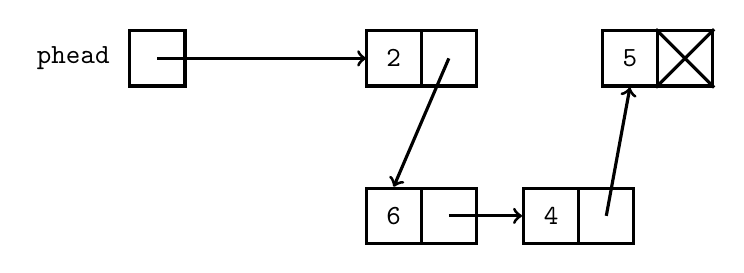
\begin{tikzpicture}

\draw (0.35, 0.35)
  node[draw, line width=0.04cm, , color=black,
       rounded corners=0cm, inner sep=0cm] {

\begin{minipage}[t][0.7cm]{0.7cm}
\mbox{}

\end{minipage}

};\draw (0.35, 0.35) node[color=black] {{\texttt{2}}};
\draw (1.0499999999999998, 0.35)
  node[draw, line width=0.04cm, , color=black,
       rounded corners=0cm, inner sep=0cm] {

\begin{minipage}[t][0.7cm]{0.7cm}
\mbox{}

\end{minipage}

};\draw (1.0499999999999998, 0.35) node[color=black] {{\texttt{}}};
\draw (0.35, -1.65)
  node[draw, line width=0.04cm, , color=black,
       rounded corners=0cm, inner sep=0cm] {

\begin{minipage}[t][0.7cm]{0.7cm}
\mbox{}

\end{minipage}

};\draw (0.35, -1.65) node[color=black] {{\texttt{6}}};
\draw (1.0499999999999998, -1.65)
  node[draw, line width=0.04cm, , color=black,
       rounded corners=0cm, inner sep=0cm] {

\begin{minipage}[t][0.7cm]{0.7cm}
\mbox{}

\end{minipage}

};\draw (1.0499999999999998, -1.65) node[color=black] {{\texttt{}}};
\draw (2.35, -1.65)
  node[draw, line width=0.04cm, , color=black,
       rounded corners=0cm, inner sep=0cm] {

\begin{minipage}[t][0.7cm]{0.7cm}
\mbox{}

\end{minipage}

};\draw (2.35, -1.65) node[color=black] {{\texttt{4}}};
\draw (3.0500000000000003, -1.65)
  node[draw, line width=0.04cm, , color=black,
       rounded corners=0cm, inner sep=0cm] {

\begin{minipage}[t][0.7cm]{0.7cm}
\mbox{}

\end{minipage}

};\draw (3.0500000000000003, -1.65) node[color=black] {{\texttt{}}};
\draw (3.35, 0.35)
  node[draw, line width=0.04cm, , color=black,
       rounded corners=0cm, inner sep=0cm] {

\begin{minipage}[t][0.7cm]{0.7cm}
\mbox{}

\end{minipage}

};\draw (3.35, 0.35) node[color=black] {{\texttt{5}}};
\draw (4.05, 0.35)
  node[draw, line width=0.04cm, , color=black,
       rounded corners=0cm, inner sep=0cm] {

\begin{minipage}[t][0.7cm]{0.7cm}
\mbox{}

\end{minipage}

};\draw (4.05, 0.35) node[color=black] {{\texttt{}}};\draw[line width=0.04cm,black,->] (1.05,0.35) to  (0.35,-1.28);
\draw[line width=0.04cm,black,->] (1.05,-1.65) to  (1.98,-1.65);
\draw[line width=0.04cm,black,->] (3.05,-1.65) to  (3.35,-0.02);
\draw[line width=0.04cm,black] (3.68,0.72) to  (4.42,-0.02);
\draw[line width=0.04cm,black] (4.42,0.72) to  (3.68,-0.02);

\draw (-2.65, 0.35)
  node[draw, line width=0.04cm, , color=black,
       rounded corners=0cm, inner sep=0cm] {

\begin{minipage}[t][0.7cm]{0.7cm}
\mbox{}

\end{minipage}

};\draw (-2.65, 0.35) node[color=black] {{\texttt{}}};\draw[line width=0.04cm,black,->] (-2.65,0.35) to  (0,0.35);

\draw (-3.7199999999999998, 0.35)
  node[draw, line width=0.04cm, , color=white,
       rounded corners=0cm, inner sep=0cm] {

\begin{minipage}[t][0.1cm]{0.1cm}
\mbox{}

\end{minipage}

};\draw (-3.7199999999999998, 0.35) node[color=black] {{\texttt{phead}}};
\end{tikzpicture}

\end{center}


